\chapter{الحفز المتجانس في الصناعة}\label{ch:b3:homogeneous-catalysis}

معظم حمض الأسيتيك في العالم، المادة الأولية لأسيتات الفينيل
وأسيتات السليلوز وحمض التيريفتاليك المنقى في القوارير البلاستيكية،
يُصنع من الميثانول وأحادي أكسيد الكربون في بضعة مصانع كبيرة جدًا. وفي كل منها، يدور
معقد للروديوم أو الإيريديوم، مذاب بتركيز منخفض في سائل
التفاعل، آلاف الدورات في الساعة، سنوات متتالية. والكيمياء نفسها
تهدرج، وتضيف CO والهيدروجين إلى الألكينات، وتبادل أطراف
الروابط المضاعفة، وتصل الحلقات العطرية، وتصنع البولي إيثيلين والبولي بروبيلين
بملايين الأطنان. ويقرأ هذا الفصل الدورات الحفزية لأهم
العمليات الصناعية بأدوات \cref{ch:b3:organometallic-bonding}:
عدّ الإلكترونات، وحالات الأكسدة، والخطوات المحددة للسرعة، وتناظر
الحفاز الذي يحدد بنية البوليمر.

\begin{recall}
قدّم مجلد السنة الثانية الخطوات الأولية للتفاعلات العضوية الفلزية
(الإضافة التأكسدية، والحذف الاختزالي، والإدخال الهجري، وحذف الهيدريد
$\beta$، والتبادل الفلزي)، والدورات الحفزية، وطلائع الحفازات، وعدد الدوران
وتردده، وقرأ دورات الهدرجة \omterm{def:b3:homogeneous-catalysis:hydroformylation}{والهدرجة الفورميلية} 
والاقتران التقاطعي؛ وعرّف أيضًا التاكتيكية والبلمرة بالنمو السلسلي، 
والتحويل والانتقائية. وعدّ \cref{ch:b3:organometallic-bonding}
الإلكترونات ووصف ربائط الكربونيل \omterm{def:b3:organometallic-bonding:carbene}{والكربين}؛
وأعطى \cref{ch:b3:complex-kinetics} حركية الإشباع؛
و\cref{ch:b3:point-groups} عناصر تناظر الجزيئات.
\end{recall}

\begin{omfigure}
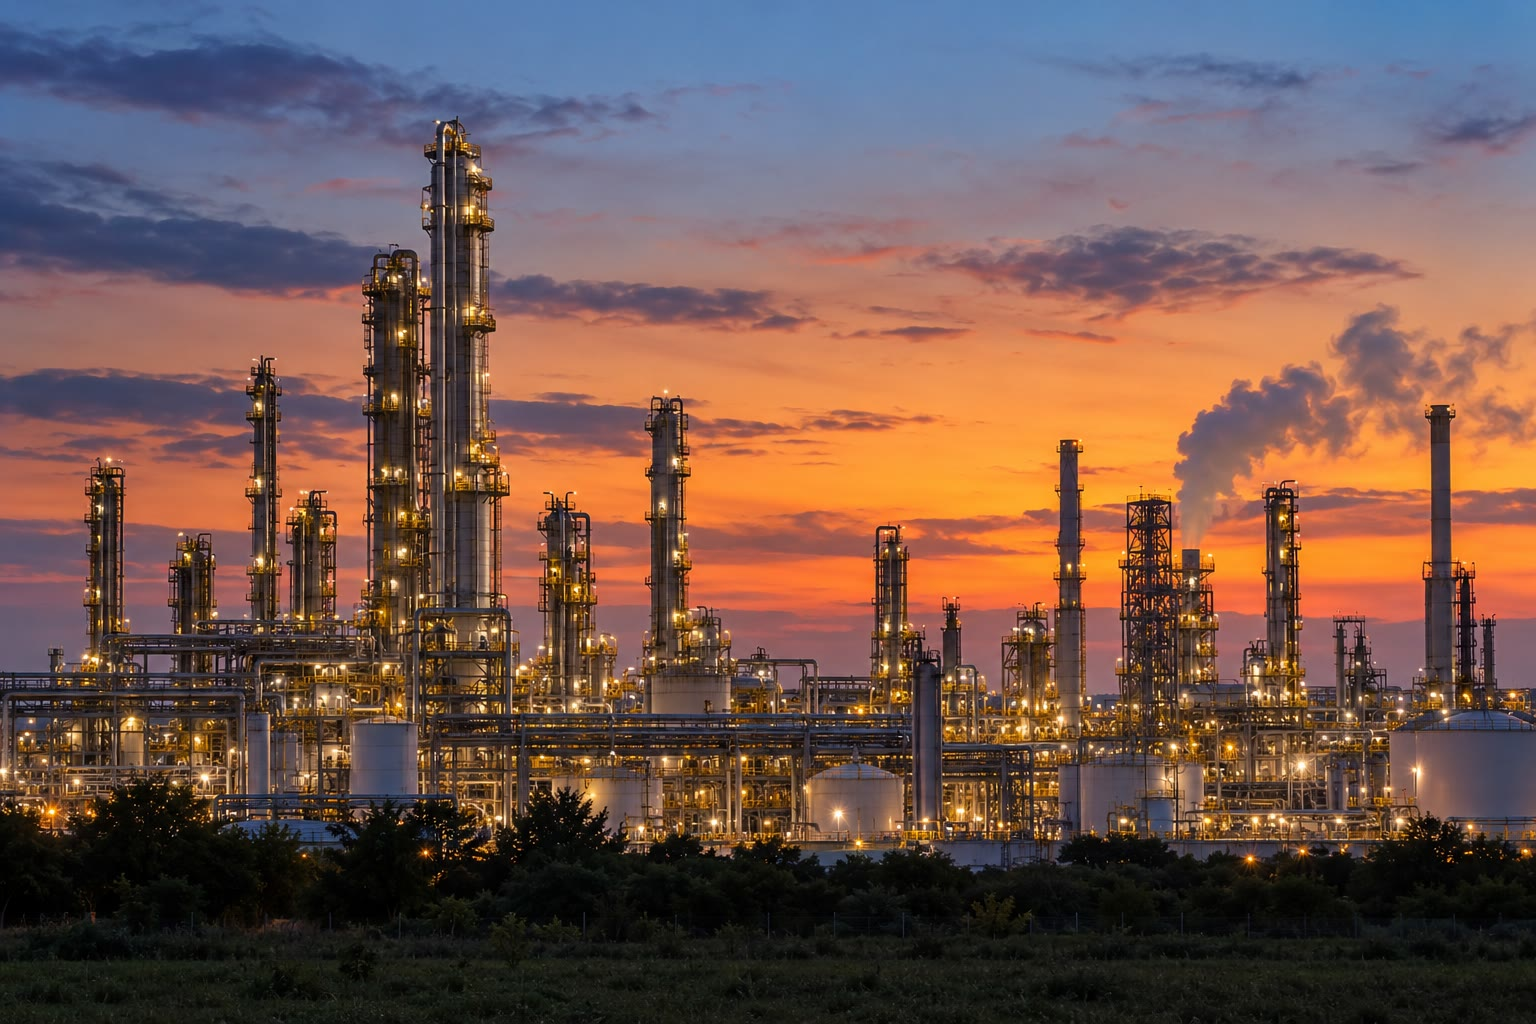
\includegraphics[width=0.6\linewidth]{images/book4/ai/b3-21-chemical-plant.jpg}

{\small مصنع كيميائي كبير عند الغسق. في وحدة \omterm{def:b3:homogeneous-catalysis:carbonylation}{الكربونلة}، يكون الحفاز
معقدًا فلزيًا مذابًا في سائل التفاعل؛ ومعظم المصنع
يفصل ويعيد التدوير.}
\end{omfigure}

\section{الهدرجة}

\begin{method}[قراءة دورة حفزية]\label{met:b3:homogeneous-catalysis:read-cycle}
\begin{enumerate}
  \item عند كل نوع، عُدّ إلكترونات التكافؤ وأعطِ حالة الأكسدة
        و$d^n$ للفلز.
  \item سمِّ كل خطوة (فقد ربيطة أو إضافتها، إضافة تأكسدية،
        إدخال، حذف) وتحقّق من أن الأعداد تتغير كما تقتضي
        (الإضافة التأكسدية: $+2$ في حالة الأكسدة وفي عدد الإلكترونات).
  \item عيّن حالة الراحة (النوع الذي يتراكم) 
        والخطوة المحددة للسرعة؛ ويُستنتج قانون السرعة من التوازنات المسبقة
        بينهما.
\end{enumerate}
\end{method}

\begin{omfigure}
\begin{tikzpicture}[font=\small, >=Stealth]
  \node (a) at (90:2.3) {\ce{RhCl(PPh3)2} \ (14, Rh$^{\mathrm I}$)};
  \node (b) at (0:3.0) {\ce{RhClH2(PPh3)2} \ (16, Rh$^{\mathrm{III}}$)};
  \node (c) at (-90:2.3) {\ce{RhClH2(RCH=CH2)(PPh3)2} \ (18)};
  \node (d) at (180:3.1) {\ce{RhClH(CH2CH2R)(PPh3)2} \ (16)};
  \draw[->, thick] (a) to[bend left=22] node[midway, above right, font=\scriptsize] {\foreignlanguage{arabic}{$+\,\ce{H2}$، إضافة تأكسدية}} (b);
  \draw[->, thick] (b) to[bend left=22] node[midway, below right, font=\scriptsize] {\foreignlanguage{arabic}{$+$ ألكين}} (c);
  \draw[->, thick] (c) to[bend left=22] node[midway, below left, font=\scriptsize] {\foreignlanguage{arabic}{إدخال هجري}} (d);
  \draw[->, thick] (d) to[bend left=22] node[midway, above left, font=\scriptsize, align=right] {\foreignlanguage{arabic}{حذف}\\ \foreignlanguage{arabic}{اختزالي: $-$ ألكان}} (a);
  \node[anchor=south] (p) at (90:3.4) {\ce{RhCl(PPh3)3} \ (16, \foreignlanguage{arabic}{طليعة الحفاز})};
  \draw[<->, black!50] (p) -- (a) node[midway, right, font=\scriptsize] {$\mp\,\ce{PPh3}$};
\end{tikzpicture}

{\small دورة مبسطة لهدرجة الألكينات بحفاز ويلكنسون
(أعداد إلكترونات التكافؤ بين قوسين). يفتح فقد فوسفين موقعًا؛ ثم
تضيف الدورة الهيدروجين، وتربط الألكين، وتُدخله في رابطة Rh--H 
وتحذف الألكان.}
\end{omfigure}

\begin{proposition}[حركية ويلكنسون]\label{prop:b3:homogeneous-catalysis:wilkinson-rate}
إذا كان $\ce{RhClL3} \rightleftharpoons \ce{RhClL2} + \mathrm L$ ($K_1$) و$\ce{RhClL2} + \ce{H2} \rightleftharpoons \ce{RhClH2L2}$ ($K_2$) توازنين
سريعين وكان تفاعل ثنائي الهيدريد مع الألكين (ثابت السرعة $k$)
هو المحدد للسرعة، فإن
\[
  v = \frac{kK_1K_2[\mathrm{Rh}]_{\mathrm{tot}}[\ce{H2}][\text{الألكين}]}{[\mathrm L] + K_1 + K_1K_2[\ce{H2}]},
\]
وهي تبلغ الإشباع بالنسبة إلى الهيدروجين وتتثبط بإضافة الفوسفين L.
\end{proposition}

\begin{proof}
$[\ce{RhClL2}] = K_1[\ce{RhClL3}]/[\mathrm L]$ و$[\ce{RhClH2L2}] = K_2[\ce{H2}][\ce{RhClL2}]$. وبكتابة $[\mathrm{Rh}]_{\mathrm{tot}}$ على أنها
مجموع الأنواع الثلاثة والحل بالنسبة إلى ثنائي الهيدريد نحصل على $[\ce{RhClH2L2}] =
K_1K_2[\ce{H2}][\mathrm{Rh}]_{\mathrm{tot}}/([\mathrm L] + K_1 + K_1K_2[\ce{H2}])$؛ والسرعة هي $k$ مضروبًا في هذا المقدار وفي تركيز
الألكين.
\end{proof}

يهدرج حفاز ويلكنسون الألكينات غير المعاقة أسرع بكثير من
المستبدلة ولا يمس مجموعات الكربونيل: وهذه انتقائية
مركز فلزي مزدحم. وتحوّل ثنائيات الفوسفين الكيرالية الكيمياء نفسها إلى
هدرجة لاتناظرية (\cref{ch:b3:asymmetric-synthesis}).

\section{عمليات الكربونلة}

\begin{definition}[الهدرجة الفورميلية]\label{def:b3:homogeneous-catalysis:hydroformylation}
\emph{الهدرجة الفورميلية}\index{هدرجة فورميلية} هي إضافة ذرة هيدروجين
ومجموعة فورميل (CHO) على رابطة مضاعفة C=C، انطلاقًا من $\ce{H2}$ وCO، فتحوّل
الألكين إلى ألدهيد فيه ذرة كربون إضافية. و\emph{نسبة الخطي إلى
المتفرع}\index{نسبة الخطي إلى المتفرع} هي نسبة الألدهيد ذي السلسلة المستقيمة
إلى الألدهيد المتفرع.
\end{definition}

استعملت العمليات الأولى $\ce{HCo(CO)4}$ عند نحو 150 إلى \qty{180}{\celsius} وضغوط
مرتفعة جدًا. أما الروديوم مع ثلاثي فينيل الفوسفين فيعمل عند نحو \qty{100}{\celsius} 
وضغوط أدنى بكثير، ويعطي نسبة أعلى من الخطي إلى المتفرع: فالفوسفينات
الضخمة تفضّل الإدخال الذي يضع الفلز على الكربون الطرفي.
ويعطي البروبين البوتانال، الذي يُهدرج إلى بوتانول أو يحوَّل إلى كحولات
الملدِّنات.

\begin{definition}[الكربونلة]\label{def:b3:homogeneous-catalysis:carbonylation}
\emph{الكربونلة}\index{كربونلة} هي إدخال مجموعة كربونيل
في جزيء بالتفاعل مع أحادي أكسيد الكربون، بحفز معقد فلزي
عبر الإدخال الهجري للجزيء CO.
\end{definition}

تجري \omterm{def:b3:homogeneous-catalysis:carbonylation}{كربونلة} الميثانول إلى حمض الأسيتيك، $\ce{CH3OH + CO -> CH3COOH}$، على
الروديوم (عملية مونسانتو) أو الإيريديوم (عملية كاتيفا) مع يوديد الميثيل
حفازًا مساعدًا: فيوديد الهيدروجين يحوّل الميثانول إلى يوديد الميثيل، والفلز
يُدخل CO في مجموعة الميثيل، ويُحلمه يوديد الأسيتيل المتكوّن،
فيتحرر HI من جديد.

\begin{omfigure}
\begin{tikzpicture}[font=\small, >=Stealth]
  \node (a) at (90:2.1) {$\ce{[M(CO)2I2]-}$ (16)};
  \node (b) at (0:2.9) {$\ce{[CH3M(CO)2I3]-}$ (18)};
  \node (c) at (-90:2.1) {$\ce{[CH3COM(CO)I3]-}$ (16)};
  \node (d) at (180:2.9) {$\ce{[CH3COM(CO)2I3]-}$ (18)};
  \draw[->, thick] (a) to[bend left=22] node[midway, above right, font=\scriptsize, align=left] {$+\,\ce{CH3I}$\\ \foreignlanguage{arabic}{إضافة تأكسدية}} (b);
  \draw[->, thick] (b) to[bend left=22] node[midway, below right, font=\scriptsize] {\foreignlanguage{arabic}{إدخال هجري}} (c);
  \draw[->, thick] (c) to[bend left=22] node[midway, below left, font=\scriptsize] {$+$ CO} (d);
  \draw[->, thick] (d) to[bend left=22] node[midway, above left, font=\scriptsize, align=right] {\foreignlanguage{arabic}{حذف اختزالي}\\ $-\,\ce{CH3COI}$} (a);
  \node[anchor=north, align=center, font=\scriptsize] at (0,-2.55) {$\ce{CH3COI + H2O -> CH3COOH + HI}$, \quad $\ce{CH3OH + HI -> CH3I + H2O}$};
\end{tikzpicture}

{\small دورة \omterm{def:b3:homogeneous-catalysis:carbonylation}{كربونلة} الميثانول من أجل $\mathrm M = \mathrm{Rh}$ (مونسانتو)؛ أعداد إلكترونات
التكافؤ بين قوسين، وحالة أكسدة الفلز I في الأعلى وIII في المواضع الأخرى.
مع الروديوم تكون الإضافة التأكسدية ليوديد الميثيل هي المحددة للسرعة. ومع
الإيريديوم (كاتيفا) تكون أسرع بكثير، ويكون الإدخال الهجري بطيئًا، 
والمعزِّزات التي تنزع يوديدًا من $\ce{[CH3Ir(CO)2I3]-}$ تسرّع الإدخال.}
\end{omfigure}

\begin{proposition}[قانون سرعة عملية الروديوم]\label{prop:b3:homogeneous-catalysis:monsanto-rate}
إذا كانت الإضافة التأكسدية ليوديد الميثيل إلى $\ce{[Rh(CO)2I2]-}$ هي المحددة للسرعة وكان
هذا المعقد هو حالة الراحة، فإن $v = k[\mathrm{Rh}]_{\mathrm{tot}}[\ce{CH3I}]$: من الرتبة صفر بالنسبة إلى CO وإلى
الميثانول.
\end{proposition}

\begin{proof}
السرعة هي سرعة الخطوة البطيئة، $k[\ce{[Rh(CO)2I2]-}][\ce{CH3I}]$، والروديوم كله تقريبًا
في حالة الراحة. ولا يدخل CO إلا بعد الخطوة البطيئة، والميثانول لا يفعل إلا أن
يجدد يوديد الميثيل، الذي يحدد تركيزَه المستقر اليوديدُ
المشحون في المفاعل لا الميثانول.
\end{proof}

تفوّق الإيريديوم على الروديوم في المصانع الجديدة لأسباب عملية: فمعقداته تبقى
في المحلول عند تراكيز أدنى من الماء، وهذا يوفّر طاقة في تجفيف
الناتج، وتعطي نواتج جانبية أقل. والتفاعل الجانبي الرئيس في كليهما هو
تفاعل إزاحة الماء--الغاز، $\ce{CO + H2O -> CO2 + H2}$، الذي يحفزه الفلز نفسه، فيُهدر
أحادي أكسيد الكربون.

\section{الإبدال الأوليفيني}

\begin{definition}[الإبدال الأوليفيني]\label{def:b3:homogeneous-catalysis:metathesis}
\emph{الإبدال الأوليفيني}\index{إبدال أوليفيني} هو تبادل
نصفي الألكيليدين بين ألكينين، $\mathrm{RCH{=}CHR + R'CH{=}CHR' \rightleftharpoons 2\,RCH{=}CHR'}$، بحفز
معقدات \omterm{def:b3:organometallic-bonding:carbene}{كربين} فلزية عبر \emph{حلقي البوتان الفلزي}\index{حلقي بوتان فلزي}،
وهو حلقة رباعية من الفلز وثلاث ذرات كربون. وصوره التخليقية هي
\emph{الإبدال المغلق للحلقة}\index{إبدال مغلق للحلقة} (RCM)، الذي يصل
طرفي ألكين في جزيء واحد في حلقة مع فقد الإيثين، 
و\emph{البلمرة بالإبدال الفاتح للحلقة}\index{بلمرة بالإبدال الفاتح للحلقة}
(ROMP) للألكينات الحلقية المتوترة، و\emph{الإبدال
التقاطعي}\index{إبدال تقاطعي} بين ألكينين مختلفين.
\end{definition}

\begin{definition}[آلية شوفان]\label{def:b3:homogeneous-catalysis:chauvin}
\emph{آلية شوفان}\index{آلية شوفان} للإبدال هي
الإضافة الحلقية $[2+2]$ لألكين إلى \omterm{def:b3:organometallic-bonding:carbene}{كربين} فلزي، $\mathrm{[M]{=}CHR}$، فتعطي
حلقي بوتان فلزيًا، يليها انفتاحه الحلقي العكسي في الاتجاه الآخر،
الذي يحرر ألكينًا جديدًا وكربينًا جديدًا.
\end{definition}

\begin{omfigure}
\setchemfig{atom sep=2.1em}
\schemestart
\chemfig{M=[:0]CHR}
\+
\chemfig{R'HC=[:0]CHR'}
\arrow{<=>}
\chemfig{M?-[:0]CHR-[:-90]CHR'-[:180]CHR'?}
\arrow{<=>}
\chemfig{M=[:0]CHR'}
\+
\chemfig{RHC=[:0]CHR'}
\schemestop
\par\vspace{10pt}

{\small \omterm{def:b3:homogeneous-catalysis:chauvin}{آلية شوفان}: يتحد \omterm{def:b3:organometallic-bonding:carbene}{كربين} فلزي وألكين في
\omterm{def:b3:homogeneous-catalysis:metathesis}{حلقي بوتان فلزي}، ينفتح في الاتجاه الآخر فيعطي كربينًا جديدًا 
وألكينًا جديدًا. وكل خطوة عكوسة: فيبلغ الإبدال توازنًا ما لم
يغادر أحد النواتج.}
\end{omfigure}

\begin{proposition}[دفع الإبدال المغلق للحلقة]\label{prop:b3:homogeneous-catalysis:metathesis-equilibrium}
من أجل إغلاق حلقة $\text{الديين} \rightleftharpoons \text{الألكين الحلقي} + \ce{C2H4}$، تدفع إزالة الإيثين من
المحلول التفاعل حتى الاكتمال؛ ويتعزز التفاعل بفضل
إنتروبيا تحرير جزيء غاز.
\end{proposition}

\begin{proof}
عند التوازن $K = [\text{الحلقة}][\ce{C2H4}]/[\text{الديين}]$: فإذا أُبقي $[\ce{C2H4}]$ منخفضًا بالتطهير بتيار غاز أو
بالتفريغ، كبر $[\text{الحلقة}]/[\text{الديين}] = K/[\ce{C2H4}]$ دون حد. ويزداد عدد الجزيئات
بواحد في التفاعل بينما الروابط المتكوّنة والمنكسرة (رابطة C=C في كل جانب)
متماثلة: $\Delta_rH^\circ \approx 0$ لحلقة غير متوترة و$\Delta_rS^\circ > 0$، فيكون $K$ ملائمًا.
\end{proof}

تجري البلمرة بالإبدال الفاتح للحلقات المتوترة، مثل النوربورنين، في الاتجاه المعاكس للسبب
المعاكس: فتحرر إجهاد الحلقة يعوّض فقد الإنتروبيا الانتقالية.
وكربينات الروثينيوم لروبرت غرابز تتحمل الماء والهواء ومعظم المجموعات
الوظيفية؛ أما ألكيليدينات الموليبدينوم والتنغستن لريتشارد شروك فأكثر نشاطًا
ويمكن جعلها انتقائية للمتماكبات المرآوية.

\section{الاقتران التقاطعي بالبلاديوم}

\begin{definition}[تفاعلات الاقتران التقاطعي]\label{def:b3:homogeneous-catalysis:cross-coupling}
\emph{تفاعل الاقتران التقاطعي}\index{تفاعل اقتران تقاطعي} يصل بين شظيتين
كربونيتين مختلفتين، هاليد عضوي وكاشف عضوي فلزي أو
ألكين، على حفاز فلزي، هو البلاديوم عادة. وفي \emph{تفاعل
هيك}\index{تفاعل هيك} يقترن هاليد أريل أو فينيل بألكين،
فيعطي ألكينًا مستبدلًا؛ وفي \emph{اقتران سوزوكي--ميياورا}\index{اقتران سوزوكي--ميياورا}
يقترن بمركب عضوي بوروني
في وجود قاعدة.
\end{definition}

\begin{omfigure}
\begin{tikzpicture}[font=\small, >=Stealth]
  \node (a) at (90:2.0) {$\mathrm{Pd^0L_2}$};
  \node (b) at (0:2.6) {$\mathrm{ArPd^{II}XL_2}$};
  \node (c) at (-90:2.0) {$\mathrm{ArPd^{II}Ar'L_2}$};
  \draw[->, thick] (a) to[bend left=25] node[midway, above right, font=\scriptsize, align=left] {$+\,$ArX\\ \foreignlanguage{arabic}{إضافة تأكسدية}} (b);
  \draw[->, thick] (b) to[bend left=25] node[midway, below right, font=\scriptsize, align=left] {$+\,\mathrm{Ar'B(OH)_2}$, \foreignlanguage{arabic}{قاعدة}\\ \foreignlanguage{arabic}{تبادل فلزي}} (c);
  \draw[->, thick] (c) to[bend left=35] node[midway, left, font=\scriptsize, align=right] {\foreignlanguage{arabic}{حذف اختزالي}\\ $-\,$Ar--Ar$'$} (a);
\end{tikzpicture}

{\small دورة سوزوكي--ميياورا: يُدخَل البلاديوم(0) في الرابطة C--X لهاليد
الأريل، ويتلقى مجموعة الأريل الثانية من حمض البورونيك المنشَّط بالقاعدة،
ويحرر ثنائي الأريل بالحذف الاختزالي.}
\end{omfigure}

\begin{method}[اختيار اقتران تقاطعي]\label{met:b3:homogeneous-catalysis:choose-coupling}
\begin{enumerate}
  \item افصل الهدف عند الرابطة C--C المراد تكوينها؛ فيصير أحد الشريكين
        الهاليد (اليوديد $>$ البروميد $>$ التريفلات $>$ الكلوريد في التفاعلية)، والآخر
        حمض البورونيك (سوزوكي--ميياورا)، أو الألكين (هيك)، أو المركب العضوي الزنكي
        (نيغيشي) أو الألكاين الطرفي مع النحاس(I) (سونوغاشيرا).
  \item فضّل زوج الشريكين الذي تكون كواشفه مستقرة ومتاحة وأقل
        سمية: أحماض البورونيك لثنائيات الأريل.
  \item اختر الربيطة من أجل أصعب خطوة: الفوسفينات الغنية بالإلكترونات والضخمة
        أو الكربينات الحلقية غير المتجانسة النيتروجينية تسرّع الإضافة التأكسدية للكلوريدات.
  \item خطّط لإزالة البلاديوم من الناتج حتى المستويات المنخفضة
        المسموح بها في الأدوية (راتنجات كاسحة، تبلور).
\end{enumerate}
\end{method}

\section{الحفز في البلمرة}

\begin{definition}[حفز تسيغلر--ناتا]\label{def:b3:homogeneous-catalysis:ziegler-natta}
\emph{حفاز تسيغلر--ناتا}\index{حفاز تسيغلر--ناتا} يبلمر
الألكينات عند ضغط منخفض؛ ويُصنع من هاليد فلز انتقالي، هو عادة
هاليد التيتانيوم، ومن مركب ألكيل ألومنيوم. و\emph{آلية كوسي--أرلمان}\index{آلية كوسي--أرلمان}
لنمو السلسلة هي تناسق
الألكين عند موقع شاغر في موضع cis من سلسلة الألكيل النامية على الفلز،
يليه إدخاله الهجري في الرابطة فلز--كربون، الذي يترك
موقعًا شاغرًا من جديد. و\emph{الحفاز الوحيد الموقع}\index{حفاز وحيد الموقع}
مراكزه النشطة كلها متماثلة، كما في حفاز ميتالوسيني جزيئي.
\end{definition}

\begin{omfigure}
\begin{tikzpicture}[font=\small, >=Stealth]
  \begin{scope}[every node/.style={inner sep=1pt}]
  % panel 1: chain and vacant site
  \node (m1) at (0,0) {M};
  \node (p1) at (-0.7,0.55) {P};
  \node (v1) at (0.7,0.55) {$\square$};
  \draw (m1) -- (p1);
  % panel 2: alkene bound side-on at the vacant site
  \node (m2) at (3.6,0) {M};
  \node (p2) at (2.9,0.55) {P};
  \node (c2a) at (4.75,1.25) {\ce{CH2}};
  \node (c2b) at (4.75,0.25) {\ce{CH2}};
  \draw (m2) -- (p2);
  \draw[double, double distance=1.6pt] (c2a) -- (c2b);
  \draw[dashed] (m2) -- (4.55,0.75);
  % panel 3: chain longer by two carbons, vacant site moved
  \node (m3) at (7.7,0) {M};
  \node (v3) at (7.0,0.55) {$\square$};
  \node (c3a) at (8.45,0.55) {\ce{CH2}};
  \node (c3b) at (8.45,1.45) {\ce{CH2}};
  \node (p3) at (7.75,1.95) {P};
  \draw (m3) -- (c3a) -- (c3b) -- (p3);
  \end{scope}
  \draw[->, thick] (1.25,0.35) -- (2.55,0.35) node[midway, above, font=\scriptsize] {$+\,\ce{C2H4}$};
  \draw[->, thick] (5.35,0.35) -- (6.3,0.35) node[midway, above, font=\scriptsize] {\foreignlanguage{arabic}{إدخال}};
\end{tikzpicture}
\par\medskip

{\small \omterm{def:b3:homogeneous-catalysis:ziegler-natta}{آلية كوسي--أرلمان} (P: سلسلة البوليمر النامية؛ $\square$: موقع
شاغر). يرتبط الألكين بجوار السلسلة ويُدخَل في الرابطة M--C
عبر حالة انتقالية رباعية الحلقة؛ فتشغل السلسلة، التي طالت بذرتي
كربون، الموقع الذي كان فيه الألكين، ويكون الموقع الشاغر قد
انتقل.}
\end{omfigure}

\begin{proposition}[التاكتيكية من تناظر الحفاز]\label{prop:b3:homogeneous-catalysis:tacticity-symmetry}
من أجل حفاز ميتالوسيني تهاجر فيه السلسلة بين موقعي تناسق
عند كل إدخال، يعطي الحفاز ذو التناظر $C_2$ بولي بروبيلين أيزوتاكتيًا
ويعطي الحفاز ذو التناظر $C_s$ بولي بروبيلين سنديوتاكتيًا.
\end{proposition}

\begin{proof}[تعليل]
يختار المحيط الكيرالي للموقع وجه البروبين الذي يُدخَل.
ففي حفاز ذي تناظر $C_2$ يتبادل الموقعان بالمحور $C_2$،
الذي يحفظ اليدوية (\cref{ch:b3:point-groups}): فيختار الموقعان كلاهما
الوجه نفسه، ويكون لمجموعات الميثيل المتعاقبة التشكيل نفسه (أيزوتاكتي).
وفي حفاز ذي تناظر $C_s$ يكون الموقعان صورتين مرآويتين: فيختاران وجهين
متعاكسين، وتتناوب التشكيلات (سنديوتاكتي). والحفاز الذي مواقعه
لاكيرالية، مثل $\ce{Cp2ZrCl2}$ غير الجسري مع الميثيل ألومينوكسان، يعطي بوليمرًا
أتاكتيًا.
\end{proof}

\begin{proposition}[توزيع شولتس--فلوري]\label{prop:b3:homogeneous-catalysis:schulz-flory}
إذا أضافت كل سلسلة نامية على \omterm{def:b3:homogeneous-catalysis:ziegler-natta}{حفاز وحيد الموقع} مونومرًا باحتمال ثابت
$p$ ونُقلت (أُنهيت) فيما عدا ذلك، فإن النسبة العددية
للسلاسل ذات $n$ وحدة هي $x_n = (1 - p)p^{n-1}$، والتشتت $M_w/M_n = 1 + p$ يؤول إلى 2 من أجل السلاسل الطويلة.
\end{proposition}

\begin{proof}
السلسلة ذات $n$ وحدة بالضبط نمت $n - 1$ مرة وتوقفت مرة واحدة:
احتمالها $p^{n-1}(1 - p)$. ومنه $\sum nx_n = 1/(1 - p)$ (المتوسط العددي)، 
والكسور الكتلية $w_n = nx_n(1 - p)$ تعطي المتوسط الكتلي $\sum nw_n = (1 + p)/(1 - p)$. 
ونسبتهما $1 + p$.
\end{proof}

\begin{omfigure}
\begin{tikzpicture}
\begin{axis}[width=0.7\linewidth, height=5.2cm, xmin=0, xmax=200, ymin=0, ymax=1.05,
  axis lines=left, xlabel={\babelsublr{$M$ / \unit{kg.mol^{-1}}}}, ylabel={\foreignlanguage{arabic}{النسبة لكل وحدة، بمقياس نسبي}},
  tick label style={font=\small}, label style={font=\small},
  legend style={font=\scriptsize, draw=none, at={(0.98,0.98)}, anchor=north east}, legend cell align=left]
\addplot[omDef, line width=1pt] table[x=M_kg, y=x] {figdata/out/bachelor-3-schulz-flory.dat};
\addplot[omThm, line width=1pt] table[x=M_kg, y expr=\thisrow{w}/0.368] {figdata/out/bachelor-3-schulz-flory.dat};
\draw[black!40, dashed] (axis cs:28.05,0) -- (axis cs:28.05,1);
\node[font=\scriptsize, anchor=west] at (axis cs:30,0.5) {$M_n$};
\legend{{\foreignlanguage{arabic}{النسبة العددية}}, {\foreignlanguage{arabic}{النسبة الكتلية، مقيسة إلى قيمتها العظمى}}}
\end{axis}
\end{tikzpicture}

{\small توزيع الكتل المولية الأكثر احتمالًا لبولي إيثيلين مصنوع على
\omterm{def:b3:homogeneous-catalysis:ziegler-natta}{حفاز وحيد الموقع} (نموذج: متوسط درجة البلمرة 1000): تنخفض النسبة
العددية أسيًا، وتبلغ النسبة الكتلية قمتها عند $M_n \approx \qty{28}{kg/mol}$؛ $M_w = 2M_n$. أما حفازات
تسيغلر--ناتا الكلاسيكية، ذات الأنواع المتعددة من المواقع، فتعطي توزيعات
أعرض.}
\end{omfigure}

\begin{inthelab}[اقتران سوزوكي وبلاديومه]
يُحرَّك بروميد الأريل وحمض البورونيك (1.2 مكافئ) وكربونات البوتاسيوم 
وبضعة أعشار في المئة من معقد فوسفيني للبلاديوم في
مزيج منزوع الغازات من التولوين والإيثانول والماء تحت النيتروجين مع التقطير الارتدادي. وبعد
المعالجة يُحرَّك ثنائي الأريل الخام مع سيليكا مُوظَّفة بالثيول
تربط البلاديوم، ثم يُرشَّح ويُبلور؛ ويُقاس البلاديوم الباقي بمطيافية
الكتلة بالبلازما.
\end{inthelab}

\begin{safety}{\ghs[0.62cm]{GHS02}\ghs[0.62cm]{GHS04}\ghs[0.62cm]{GHS06}\ghs[0.62cm]{GHS08}}
% ledger: ghs4:MeI, ghs:CO
يوديد الميثيل: سام بالاستنشاق والابتلاع، ضار بملامسة الجلد، يُشتبه في أنه
مسرطن، متطاير؛ يُتداول تحت ساحبة الأبخرة. أحادي أكسيد الكربون: شديد
الاشتعال للغاية، سام بالاستنشاق، قد يضر بالجنين، عديم الرائحة؛ يُستعمل
مع أجهزة كشف ثابتة وأجهزة إنذار.
\end{safety}

\begin{history}[تسيغلر وناتا والإبدال]
وجد كارل تسيغلر في سنة 1953 أن كلوريد التيتانيوم ومركبات ألكيل الألومنيوم
تبلمر الإيثين عند الضغط الجوي، ووجد جوليو ناتا في سنة 1954 أن هذه
الحفازات تصنع بولي بروبيلين منتظمًا فراغيًا؛ وتقاسما جائزة نوبل في
الكيمياء لسنة 1963. واقترح إيف شوفان آلية \omterm{def:b3:homogeneous-catalysis:metathesis}{حلقي البوتان الفلزي} في
الإبدال سنة 1971؛ ونال مع روبرت غرابز وريتشارد شروك، اللذين صنعا حفازات
إبدال محددة البنية، جائزة نوبل في الكيمياء لسنة 2005.
\end{history}

\section{تمارين}

\begin{exercise}[$\star$]\label{exo:b3:homogeneous-catalysis:1}
أعطِ عدد إلكترونات التكافؤ وحالة أكسدة الروديوم في كل خطوة
من دورة ويلكنسون في الشكل.
\end{exercise}

\begin{exercise}[$\star$]\label{exo:b3:homogeneous-catalysis:2}
سمِّ الألدهيدين المتكوّنين \omterm{def:b3:homogeneous-catalysis:hydroformylation}{بالهدرجة الفورميلية} للبروبين. أيهما
الخطي؟
\end{exercise}

\begin{exercise}[$\star$]\label{exo:b3:homogeneous-catalysis:3}
يخضع ثنائي أليل مالونات ثنائي الإيثيل، $\ce{(CH2=CHCH2)2C(CO2Et)2}$، \omterm{def:b3:homogeneous-catalysis:metathesis}{لإبدال مغلق للحلقة}.
أعطِ الناتج وحجم حلقته.
\end{exercise}

\begin{exercise}[$\star$]\label{exo:b3:homogeneous-catalysis:4}
أعطِ ناتج \omterm{def:b3:homogeneous-catalysis:cross-coupling}{تفاعل هيك} بين اليودوبنزين وأكريلات الميثيل، 
وتشكيله.
\end{exercise}

\begin{exercise}[$\star\star$]\label{exo:b3:homogeneous-catalysis:5}
انطلاقًا من دورة عملية الروديوم، استنتج قانون سرعتها، وفسّر
لماذا لا يغيّر تحويل الميثانول السرعة إلى أن يكاد يكتمل.
\end{exercise}

\begin{exercise}[$\star\star$]\label{exo:b3:homogeneous-catalysis:6}
اقترح فصلين من نوع سوزوكي--ميياورا للمركب 4-ميثيل ثنائي الفينيل واختر أحدهما.
\end{exercise}

\begin{exercise}[$\star\star$]\label{exo:b3:homogeneous-catalysis:7}
تنبّأ بتاكتيكية البولي بروبيلين المصنوع بحفاز زركونيوم ثنائي (إنديينيل) جسري ذي تناظر $C_2$،
وبحفاز ذي تناظر $C_s$، وبالمركب $\ce{Cp2ZrCl2}$ غير الجسري.
\end{exercise}

\begin{exercise}[$\star\star$]\label{exo:b3:homogeneous-catalysis:8}
مع \qty{0.10}{mol\%} من الحفاز، تبلغ هدرجة تحويلًا قدره 98\,\% في \qty{2.0}{h}.
احسب عدد الدوران ومتوسط تردد الدوران.
\end{exercise}

\begin{exercise}[$\star\star$]\label{exo:b3:homogeneous-catalysis:9}
ارسم الوحدة المتكررة للبوليمر المصنوع بالإبدال الفاتح لحلقة
النوربورنين، وفسّر لماذا يكتمل التفاعل.
\end{exercise}

\begin{exercise}[$\star\star\star$]\label{exo:b3:homogeneous-catalysis:10}
يعطي \omterm{def:b3:homogeneous-catalysis:ziegler-natta}{حفاز وحيد الموقع} سلاسل مع $p = 0.9995$. احسب درجة البلمرة
المتوسطة العددية والتشتت. ولماذا يكون بوليمر تسيغلر--ناتا
أعرض توزيعًا؟
\end{exercise}

\begin{exercise}[$\star\star\star$]\label{exo:b3:homogeneous-catalysis:11}
بيّن انطلاقًا من قانون سرعة ويلكنسون أن السرعة من الرتبة الأولى بالنسبة إلى $\ce{H2}$ عند الضغط المنخفض
ومستقلة عنه عند الضغط المرتفع، وأن إضافة الفوسفين تبطّئ
التفاعل.
\end{exercise}

\begin{exercise}[$\star\star\star$]\label{exo:b3:homogeneous-catalysis:12}
فسّر لماذا ترفع الفوسفينات الضخمة \omterm{def:b3:homogeneous-catalysis:hydroformylation}{نسبة الخطي إلى المتفرع} في \omterm{def:b3:homogeneous-catalysis:hydroformylation}{الهدرجة الفورميلية}
بالروديوم، ولماذا تهم النسبة المرتفعة في كحولات الملدِّنات المصنوعة
من الألدهيدات.
\end{exercise}

\section{مسألة: من الميثانول إلى الخل}

\begin{problem}[{مسألة نهاية الأسبوع --- من الميثانول إلى الخل على دورة إيريديوم:
أعداد الدورة وخطواتها، وخطوتها المحددة للسرعة ومعزِّزاتها، 
وتردد الدوران في مصنع، وأحادي أكسيد الكربون المفقود في تفاعل إزاحة
الماء--الغاز}]
\label{pb:b3:homogeneous-catalysis:1}
% ledger: aw:Ir, aw:C, aw:H, aw:O
ينتج مصنع لحمض الأسيتيك (معطيات المسألة) $\qty{5.0e5}{t}$ من حمض الأسيتيك في السنة
في \qty{8000}{h} من التشغيل، مع \qty{200}{m^3} من سائل التفاعل يحوي \qty{5.0}{mmol/L} من
الإيريديوم. وانتقائيته بالنسبة إلى أحادي أكسيد الكربون 94\,\%: والباقي يحوّله
تفاعل إزاحة الماء--الغاز.

\medskip\noindent\textbf{الجزء الأول --- الدورة.}
\begin{enumerate}
  \item عُدّ إلكترونات $\ce{[Ir(CO)2I2]-}$ وأعطِ حالة أكسدته.
  \item الإضافة التأكسدية للمركب $\ce{CH3I}$: الناتج، والعدد، وحالة الأكسدة؟
  \item فقد يوديد وإضافة CO: أي معقد متعادل يتكوّن؟
  \item الإدخال الهجري: الناتج والعدد؟
  \item إضافة يوديد، ثم الحذف الاختزالي ليوديد الأسيتيل: ماذا
        يتجدد؟
  \item اكتب الخطوتين العضويتين اللتين تغلقان الدورة بالماء والميثانول.
  \item اكتب التفاعل الإجمالي.
\end{enumerate}

\medskip\noindent\textbf{الجزء الثاني --- الحركية.}
\begin{enumerate}[resume]
  \item أي خطوة هي المحددة للسرعة مع الإيريديوم، وبمَ يختلف ذلك عن
        الروديوم؟
  \item كيف تسرّع المعزِّزات التي تأسر اليوديد الدورة؟
  \item بأي اعتماد على تركيز اليوديد يتنبأ ذلك؟
  \item لماذا تكون السرعة مستقلة عن تركيز الميثانول؟
\end{enumerate}

\medskip\noindent\textbf{الجزء الثالث --- المصنع.}
\begin{enumerate}[resume]
  \item احسب كمية حمض الأسيتيك المصنوعة في السنة.
  \item احسب الكمية في الساعة.
  \item احسب كمية الإيريديوم في المفاعل، وكتلته.
  \item احسب تردد الدوران.
  \item احسب عدد الدوران في السنة.
  \item احسب المردود الزمكاني بالكيلوغرام لكل متر مكعب في الساعة.
\end{enumerate}

\medskip\noindent\textbf{الجزء الرابع --- إزاحة الماء--الغاز.}
\begin{enumerate}[resume]
  \item اكتب تفاعل إزاحة الماء--الغاز.
  \item احسب CO المستهلك لكل مول من حمض الأسيتيك.
  \item احسب \ce{CO2} المتكوّن لكل مول من حمض الأسيتيك.
  \item احسب كتلة \ce{CO2} المنبعثة لكل طن من حمض الأسيتيك.
  \item لماذا يفيد التشغيل عند تركيز أدنى للماء، وما الذي يحدّه؟
  \item ما الناتج الآخر لتفاعل الإزاحة، ولماذا يمثل مشكلة في
        المفاعل؟
  \item اذكر النتيجة: تردد الدوران لحفاز الإيريديوم.
\end{enumerate}
\end{problem}
